\documentclass[12pt, twoside]{article}
% \documentclass[12pt, twoside]{article}
\usepackage[letterpaper, margin=1in, headsep=0.2in]{geometry}
\setlength{\headheight}{0.6in}
%\usepackage[english]{babel}
\usepackage[utf8]{inputenc}
\usepackage{microtype}
\usepackage{amsmath}
\usepackage{amssymb}
%\usepackage{amsfonts}
\usepackage[nomessages]{fp} %\FPeval{\var-name}{2*sin(pi/6)}
\usepackage{siunitx} %units in math. eg 20\milli\meter
\usepackage{yhmath} % for arcs, overparenth command
\usepackage{tikz} %graphics
\usetikzlibrary{quotes, angles, arrows, arrows.meta}
\usepackage{graphicx} %consider setting \graphicspath{{images/}}
\usepackage{parskip} %no paragraph indent
\usepackage{enumitem}
\usepackage{multicol}
\usepackage{venndiagram}

\usepackage{fancyhdr}
\pagestyle{fancy}
\fancyhf{}
\renewcommand{\headrulewidth}{0pt} % disable the underline of the header
\raggedbottom
\hfuzz=2mm %suppresses overfull box warnings

\usepackage{hyperref}
\usepackage{float}

\fancyhead[LE]{\thepage}
\fancyhead[RO]{\thepage \\ First and last name: \hspace{2.5cm} \,\\ Section: \hspace{2.5cm} \,}
\fancyhead[LO]{BECA/Huson/Geometry: Construction \\* 15 November 2024}

\begin{document}
\subsubsection*{3.5 Classwork: Dilation \hfill CCSS.HSG.SRT.B.5}
\begin{enumerate}
  \item Dilate the triangle $ABC \rightarrow A'B'C'$ by a factor of $k=2$ centered at the origin.
  \begin{multicols}{2}
    \begin{tikzpicture}[scale=.7]
      \draw [help lines] (-1,-4) grid (9,5);
      \draw [thick, ->] (-1.2,0) -- (9.4,0) node [below right] {$x$};
      \draw [thick, ->] (0,-4.2)--(0,5.4) node [left] {$y$};
      \draw [thick] (0,0)node[below left]{$A$}--
       (3,-1)node[below left]{$C$}--
         (4,2)node[above left]{$B$}--cycle;
    \end{tikzpicture}

    Complete the table of coordinate mappings.\\[0.5cm]
    $A(0,0) \rightarrow A'(0,0)$ \vspace{3cm}
  \end{multicols}
  
\item A dilation centered at $A$ with a scale factor of $\displaystyle k=\frac{3}{2}$ maps $\triangle ABC \rightarrow \triangle ADE$. 
\begin{multicols}{2}
Given $AB=10$, $BC=6$, and $AC=8$. Complete the table and mark the diagram. 

$\displaystyle AD= \frac{3}{2} \times 10 =$\\[1cm]
$DE=$\\[1cm]
$AE=$\\
\begin{flushright}
  \begin{tikzpicture}[scale=1]
    \draw [thick]
    (0,0)node[left]{$A$}--
    (0:7.5)node[below]{$D$}--
    (40:6)node[above]{$E$}--cycle;
    \draw [thick]
    (0:5)node[below]{$B$}--
    (40:4)node[above left]{$C$};
    \node at (0:2.5)[below]{$10$};
    \node at (20:4.3)[right]{$6$};
    \node at (42:2)[above]{$8$};
  \end{tikzpicture}
\end{flushright}
\end{multicols}

\begin{multicols}{2}
[\item Definition: $\triangle LGA \sim \triangle JFK$ if and only if all three corresponding angles are congruent.] \vspace{0.5cm}
  \begin{tikzpicture}[scale=0.9]
    \coordinate [label=above left:$G$](A) at (80:2);
    \coordinate [label=left:$L$](B) at (0, 0);
    \coordinate [label=right:$A$](C) at (0:3);
    \draw [thick] (A)--(B)--(C)--cycle;
    \draw [thick, xshift=3cm, yshift=1.5cm, scale=1.3, rotate=-30] (80:2) node[above]{$F$}--
    (0,0) node[above left]{$J$}--
    (0:3) node[right]{$K$}--cycle;
  \end{tikzpicture}\\
  Are the given triangles similar?
  \begin{enumerate}
    \item $m\angle L =80^\circ$, $m\angle A =43^\circ$\\[0.5cm]
    Find $m\angle G =$ \rule{2cm}{0.15mm}
    \item $m\angle J =80^\circ$, $m\angle F =57^\circ$\\[0.5cm]
    Find $m\angle K =$ \rule{2cm}{0.15mm}
  \end{enumerate}
\end{multicols}

\newpage
\begin{multicols}{2}
[\item Given $\triangle ABC \sim \triangle DEF$. Mark the legs $AB=12$, $BC=18$, $AC=9$, and $DE=15$.] \vspace{0.5cm}
    \begin{tikzpicture}[scale=1.2]
      \coordinate [label=above left:$B$](A) at (80:2.5);
      \coordinate [label=below:$A$](B) at (0, 0);
      \coordinate [label=below:$C$](C) at (0:2);
      \draw [thick] (A)--(B)--(C)--cycle;
      \draw [thick, xshift=3cm, yshift=0cm, scale=1.3, rotate=0] (80:2.5) node[above]{$E$}--
      (0,0) node[below]{$D$}--
      (0:2) node[below]{$F$}--cycle;
    \end{tikzpicture}\\
    Find the scale factor and missing sides.
    \begin{enumerate}
      \item $\displaystyle k=\frac{DE}{AB}=$ \vspace{0.5cm}
      \item $\displaystyle EF= k \times BC =$ \vspace{0.5cm}
      \item $DF=$
    \end{enumerate}
  \end{multicols} \vspace{1cm}

\item Triangle $ABC$ is dilated with a scale factor of $k=2.5$ centered at $A$, yielding $\triangle ADE$, as shown. Given $AB=6$, $AC=5$, and $DE=17.5$. \\[0.25cm] Find $AD$, $AE$, and $BC$. Then find $BD$ and $CE$.
\begin{flushright}
\begin{tikzpicture}[scale=0.8]
  \draw [thick]
  (0,0)node[above]{$A$}--
  (-130:8.75)node[below]{$D$}--
  (-60:7.5)node[below]{$E$}--cycle;
  \draw [thick]
  (-130:3.5)node[above left]{$B$}--
  (-60:3)node[above right]{$C$};
  \node at (-150:1.75)[below]{$6$};
  \node at (-55:1.5)[right]{$5$};
  \node at (-95:7.5)[above]{$17.5$};
\end{tikzpicture}
\end{flushright} \vspace{2cm}

\item A dilation centered at the origin and scale factor $k$ maps $P(2,5) \rightarrow P'(5,12.5)$. Find $k$.


\end{enumerate}
\end{document}